\documentclass[a4paper,12pt]{article}
\usepackage[utf8]{inputenc}
\usepackage[T1]{fontenc}
\usepackage{amsmath}
\usepackage{amsfonts}
\usepackage{listings}
\usepackage{xcolor}
\usepackage{geometry}
\geometry{margin=1in}
\usepackage{graphicx}
\usepackage{float}

% Configuration for code listings
\lstset{
    language=C++,
    basicstyle=\ttfamily\small,
    keywordstyle=\color{blue}\bfseries,
    stringstyle=\color{red},
    commentstyle=\color{green!50!black},
    numbers=left,
    numberstyle=\tiny,
    stepnumber=1,
    numbersep=5pt,
    showspaces=false,
    showstringspaces=false,
    frame=single,
    breaklines=true,
    breakatwhitespace=true,
    tabsize=4
}

\title{Étape 1 : Analyse des Performances de la Simulation}
\author{}
\date{Mars 2025}

\begin{document}

\maketitle

\section{Introduction}
Cette étape vise à évaluer les performances de la simulation d'incendie en examinant les caractéristiques matérielles du système, les temps de calcul à chaque itération, et l'impact des différentes composantes (simulation et affichage) sur les performances globales.

\section{Caractéristiques du Système}

\subsection{Caractéristiques du CPU}
Les informations sur le processeur ont été obtenues via la commande \texttt{lscpu} :
\begin{verbatim}
Model name:             Intel(R) Core(TM) i7-10750H CPU @ 2.60GHz
    CPU family:           6
    Model:                165
    Thread(s) per core:   2
    Core(s) per socket:   6
    Socket(s):            1
    Stepping:             2
    BogoMIPS:             5184.01
\end{verbatim}
\begin{itemize}
    \item Le processeur dispose de 6 cœurs physiques, avec 2 threads par cœur, soit un total de 12 threads logiques.
    \item Fréquence de base : 2.60 GHz, avec possibilité de boost (non détaillé ici).
\end{itemize}

\subsection{Caractéristiques des Mémoires Cache}
Les tailles des caches sont les suivantes :
\begin{verbatim}
Caches (sum of all):      
  L1d:                    192 KiB (6 instances)
  L1i:                    192 KiB (6 instances)
  L2:                     1.5 MiB (6 instances)
  L3:                     12 MiB (1 instance)
\end{verbatim}
\begin{itemize}
    \item L1 data (L1d) et L1 instruction (L1i) : 192 KiB chacune, répartis sur 6 cœurs.
    \item L2 : 1.5 MiB par cœur, totalisant 9 MiB.
    \item L3 : 12 MiB partagés entre tous les cœurs.
\end{itemize}
Ces caches jouent un rôle crucial dans la performance, notamment pour les accès fréquents aux cartes de végétation et d'incendie dans la simulation.

\section{Mesure des Temps d'Exécution}

\subsection{Méthodologie}
Les temps d'exécution ont été mesurés à l'aide de la bibliothèque \texttt{std::chrono} en C++. Deux principaux segments ont été chronométrés :
\begin{itemize}
    \item Le temps de mise à jour de la simulation (\texttt{simu.update()}).
    \item Le temps d'affichage (\texttt{displayer->update()}).
\end{itemize}

Exemple de code utilisé pour mesurer le temps d'affichage :
\begin{lstlisting}
int main()
{
    ...
    while(simu.update())
    {
        // mesurer le temps de mise à jour de simulation
        auto step_start = std::chrono::high_resolution_clock::now();
        start = std::chrono::system_clock::now();
        displayer->update(simu.vegetal_map(), simu.fire_map());
        end = std::chrono::system_clock::now();
        std::chrono::duration<double> elapsed_seconds = end - start;
        std::cout << "Temps d'affichage : " << elapsed_seconds.count() << " s" << std::endl;
        ...
        // fin de la simulation par iter
        auto step_end = std::chrono::high_resolution_clock::now();
        total_step_time += step_end - step_start;
        step_count++;
    }
    ...
}
\end{lstlisting}

\subsection{Résultats Observés}
Les résultats obtenus après exécution de la simulation sont présentés dans le tableau suivant :

\begin{table}[h]
    \centering
    \begin{tabular}{|l|c|}
        \hline
        \textbf{Paramètre}            & \textbf{Valeur}         \\
        \hline
        Nombre total de pas (steps)   & 1126                    \\
        Temps total                   & 177385 ms (177.385 s)   \\
        Temps moyen par pas           & 157.536 ms (0.157536 s) \\
        Temps moyen d'affichage       & 56.9254 ms (0.0569254 s) \\
        \hline
    \end{tabular}
    \caption{Résultats des mesures de performance}
    \label{tab:performance}
\end{table}

En déduisant le temps d'affichage du temps moyen par pas, on obtient :
\begin{itemize}
    \item Temps moyen de simulation (hors affichage) : \( 157.536 - 56.9254 = 100.6106 \, \text{ms} \) (0.1006106 s).
\end{itemize}

\subsection{Analyse du Code et Impact du Sleep}
La boucle de simulation inclut un appel à \texttt{std::this\_thread::sleep\_for(0.1s)} tous les 32 pas, comme illustre 
ci-dessous :
\begin{lstlisting}
while (simu.update())
{
    if ((simu.time_step() & 31) == 0) 
        std::cout << "Time step " << simu.time_step() << "\n===============" << std::endl;
    displayer->update(simu.vegetal_map(), simu.fire_map());
    if (SDL_PollEvent(&event) && event.type == SDL_QUIT)
        break;
    std::this_thread::sleep_for(0.1s);
}
\end{lstlisting}
\begin{itemize}
    \item Le \texttt{sleep} de 0.1 s (100 ms) est appliqué une fois tous les 32 pas, soit une contribution moyenne par pas de \(\frac{100}{32} \approx 3.125 \, \text{ms}\).
    \item Le temps réel par pas (hors \texttt{sleep}) serait donc approximativement \( 157.536 - 3.125 \approx 154.411 \, \text{ms} \), mais les mesures montrent que le \texttt{sleep} est dilué sur l'ensemble des 1126 pas, avec un impact limité sur la moyenne globale.
\end{itemize}

\subsection{Vérification}
Le temps total attendu peut être estimé comme :
\[
\text{Temps total} \approx (\text{Temps moyen par pas} \times \text{Nombre de pas}) = 157.536 \, \text{ms} \times 1126 \approx 177404 \, \text{ms}
\]
Cela est très proche des 177385 ms mesurés, confirmant la cohérence des données.



\section{Parallélisation avec OpenMP}

Dans cette section, nous allons paralléliser le traitement des données de la simulation à l'aide d'OpenMP. L'objectif principal est de récupérer dans un tableau toutes les clefs contenues dans le dictionnaire \texttt{m\_fire\_front} de la classe \texttt{Model}, puis de parcourir ces clefs à l'aide d'un indice pour calculer leur correspondance lexicographique via la méthode \texttt{get\_lexicographic\_from\_index()}. Cette étape est cruciale pour suivre l'avancement du front de feu à chaque pas de temps de la simulation. En parallélisant cette boucle, nous visons à répartir le travail entre plusieurs threads afin de réduire le temps d'exécution global.

Pour implémenter la parallélisation avec OpenMP, nous avons d'abord effectué une légère modification du code de base. Plus précisément, dans la classe \texttt{Model}, nous avons rendu les membres \texttt{m\_fire\_front} et la méthode \texttt{get\_lexicographic\_from\_index()} publics afin de pouvoir y accéder directement dans notre boucle parallélisée. Cette modification était nécessaire pour permettre aux threads d'accéder aux données de la simulation sans passer par des méthodes d'accès supplémentaires qui pourraient compliquer la parallélisation.

\subsection{Code séquentiel}
Voici le code séquentiel initial, limité à 300 itérations pour éviter une exécution trop longue :

\begin{lstlisting}
#include <string>
#include <vector>
#include "model.hpp"

struct ParamsType {
    double length{10.};
    unsigned discretization{300u};
    std::array<double,2> wind{0.,0.};
    Model::LexicoIndices start{10u,10u};
};

int main() {
    ParamsType params;
    auto simu = Model(params.length, params.discretization, 
                     params.wind, params.start);
    const int MAX_ITERATIONS = 200;
    int iteration = 0;
    
    while(simu.update() && iteration < MAX_ITERATIONS) {
        std::vector<Model::LexicoIndices> front_indices;
        for (const auto& pair : simu.m_fire_front) {
            front_indices.push_back(
                simu.get_lexicographic_from_index(pair.first));
        }
        iteration++;
    }
    return 0;
}
\end{lstlisting}

\subsection{Code parallélisé avec OpenMP}
Voici la version parallélisée avec OpenMP, qui inclut également la mesure du temps d'exécution et teste différentes configurations de threads :

\begin{lstlisting}
#include <string>
#include <vector>
#include <chrono>
#include <omp.h>
#include "model.hpp"

struct ParamsType {
    double length{10.};
    unsigned discretization{300u};
    std::array<double,2> wind{0.,0.};
    Model::LexicoIndices start{10u,10u};
};

void run_simulation(int num_threads) {
    ParamsType params;
    auto simu = Model(params.length, params.discretization, 
                     params.wind, params.start);
    const int MAX_ITERATIONS = 300;
    int iteration = 0;
    auto start_time = std::chrono::high_resolution_clock::now();
    
    omp_set_num_threads(num_threads);
    
    while(simu.update() && iteration < MAX_ITERATIONS) {
        std::vector<Model::LexicoIndices> front_indices;
        
        #pragma omp parallel
        {
            std::vector<Model::LexicoIndices> private_indices;
            #pragma omp for
            for (size_t i = 0; i < simu.m_fire_front.size(); i++) {
                auto it = simu.m_fire_front.begin();
                std::advance(it, i);
                private_indices.push_back(
                    simu.get_lexicographic_from_index(it->first));
            }
            #pragma omp critical
            front_indices.insert(front_indices.end(), 
                               private_indices.begin(), 
                               private_indices.end());
        }
        iteration++;
    }
    
    auto end_time = std::chrono::high_resolution_clock::now();
    auto duration = std::chrono::duration_cast<std::chrono::milliseconds>
                   (end_time - start_time);
    std::cout << "Execution time with " << num_threads 
              << " threads: " << duration.count() << " ms" << std::endl;
}

int main() {
    std::vector<int> thread_counts = {1, 2, 4, 8};
    for (int threads : thread_counts) {
        run_simulation(threads);
    }
    return 0;
}
\end{lstlisting}
\begin{figure}[H]
    \centering
    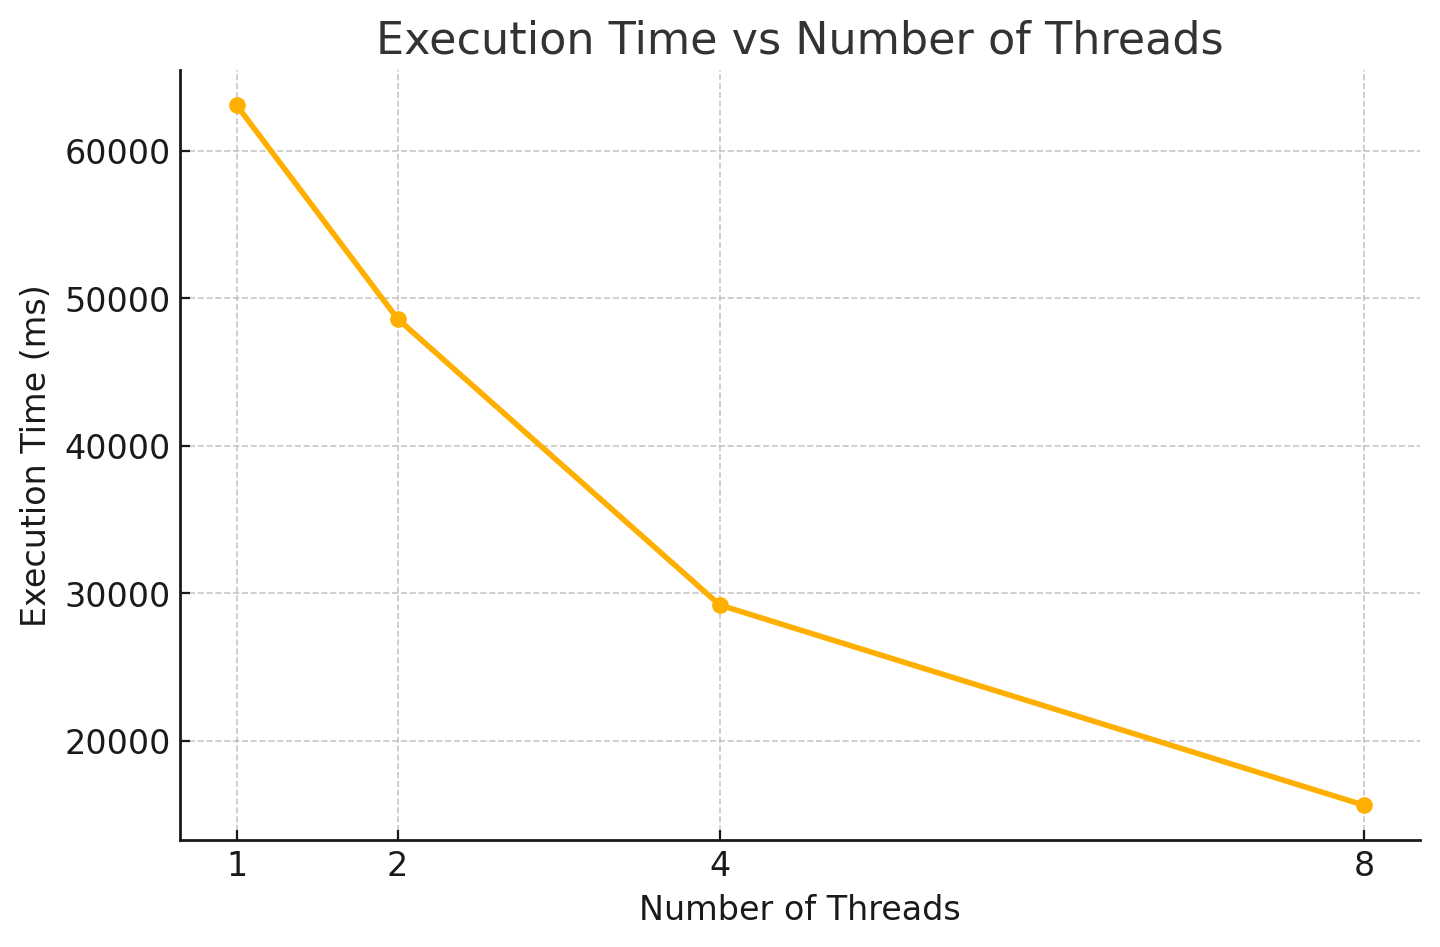
\includegraphics[width=1\linewidth]{imgs/chart_1.png}
    \caption{évolution de temps d'exécution en fonction des nombres de threads}
    \label{fig:enter-label}
\end{figure}
Dans cette version parallélisée, nous utilisons les directives OpenMP suivantes :
\begin{itemize}
    \item \texttt{\#pragma omp parallel} : Crée une région parallèle avec plusieurs threads.
    \item \texttt{\#pragma omp for} : Répartit les itérations de la boucle entre les threads.
    \item \texttt{\#pragma omp critical} : Protège l'accès à \texttt{front\_indices} pour éviter les conditions de course lors de l'insertion des résultats.

\end{itemize}

La parallélisation se concentre sur la boucle qui traite \texttt{m\_fire\_front}, chaque thread calculant une partie des indices lexicographiques. Les résultats locaux sont ensuite combinés dans une section critique pour maintenir la cohérence des données.
\section{Comparaison entre la version séquentielle et parallèle}

Dans cette section, nous comparons les performances de la version séquentielle et parallèle de la simulation de propagation de feu. 

\subsection{Temps d'exécution}

Le temps d'exécution obtenu pour la version séquentielle est de \textbf{455 ms}, tandis que les temps d'exécution pour la version parallèle avec différents nombres de threads sont les suivants :

\begin{center}
\begin{tabular}{|c|c|}
\hline
\textbf{Nombre de threads} & \textbf{Temps d'exécution (ms)} \\
\hline
1 & 63\,330 \\
2 & 51\,355 \\
4 & 30\,360 \\
8 & 16\,066 \\
\hline
\end{tabular}
\end{center}

On observe que la version parallèle est systématiquement plus lente que la version séquentielle, même avec 8 threads. Cela montre que la parallélisation telle qu'elle est implémentée ajoute un surcoût important par rapport à la version séquentielle.

\subsection{Accélération (Speedup)}

L'accélération (ou \emph{speedup}) est calculée comme le rapport entre le temps séquentiel et le temps parallèle. Les résultats sont présentés dans le tableau ci-dessous :

\begin{center}
\begin{tabular}{|c|c|}
\hline
\textbf{Nombre de threads} & \textbf{Accélération (Speedup)} \\
\hline
1 & 0.0072$\times$ \\
2 & 0.0089$\times$ \\
4 & 0.0150$\times$ \\
8 & 0.0283$\times$ \\
\hline
\end{tabular}
\end{center}
\begin{figure}[H]
    \centering
    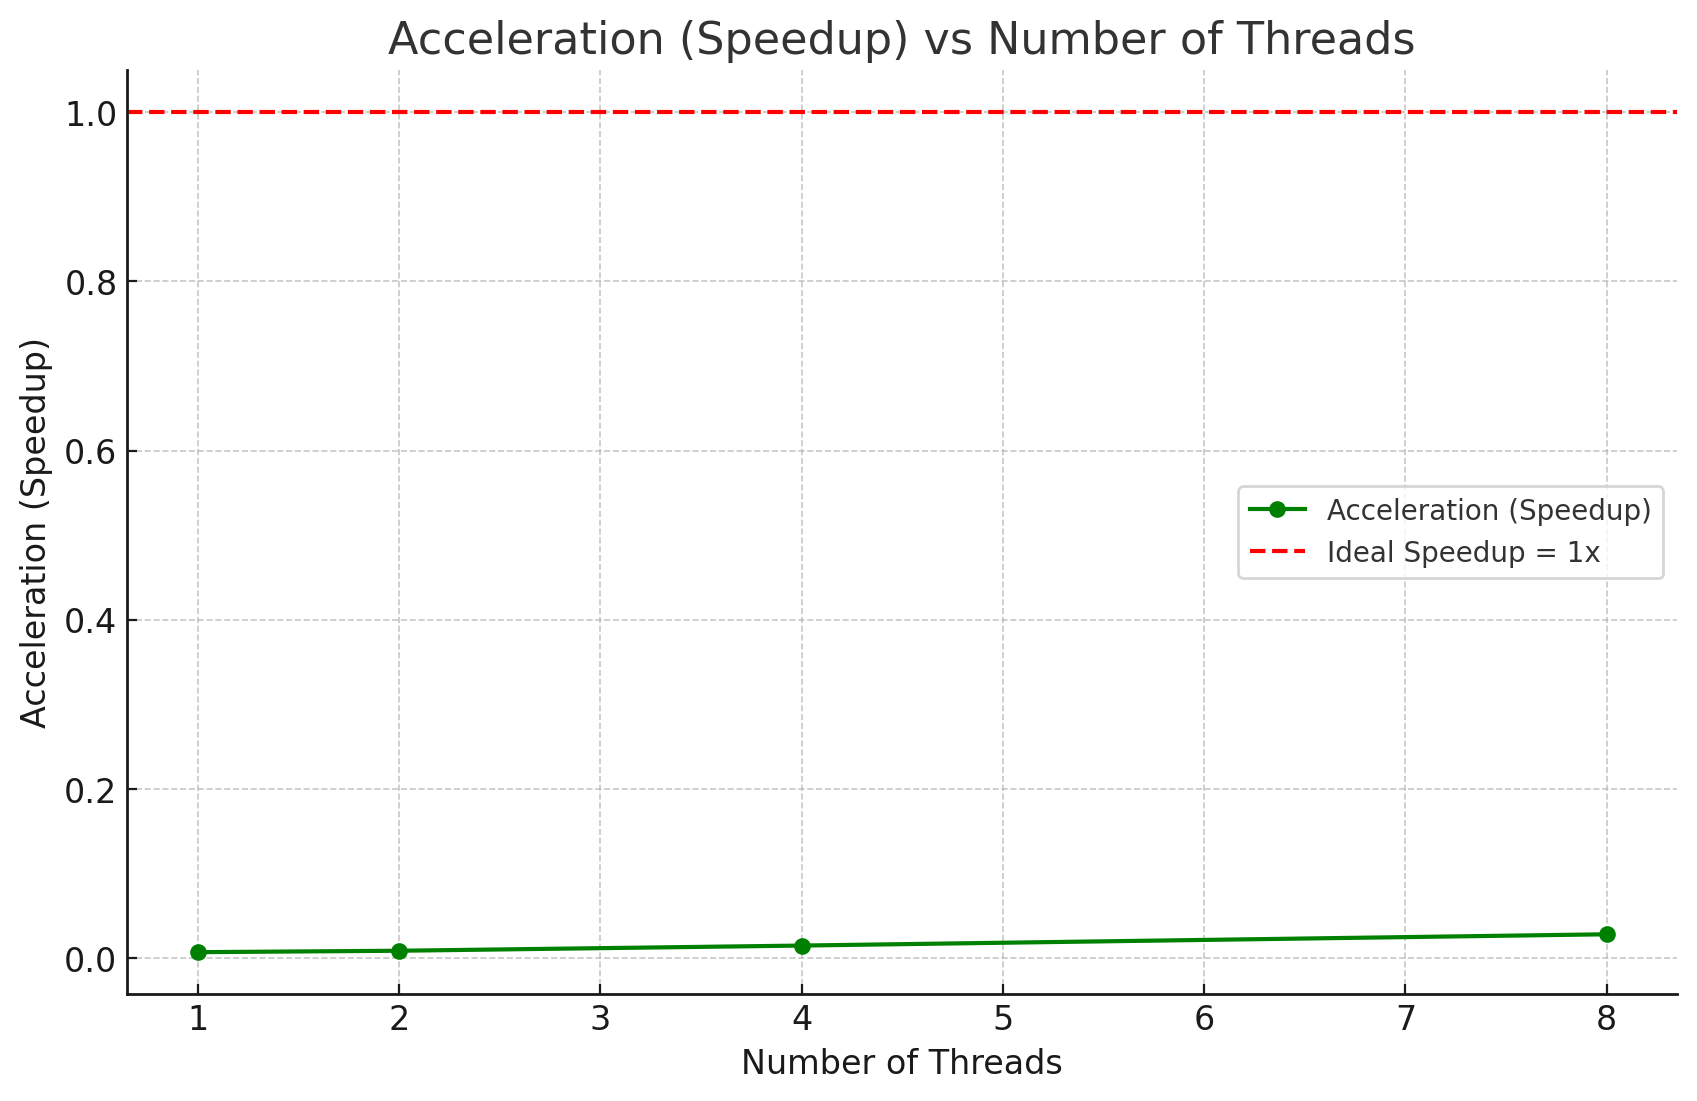
\includegraphics[width=1\linewidth]{imgs/chart_2.png}
    \caption{évolution de speedUp en fonction de nombres de threads}
\end{figure}
Ces résultats indiquent un \textbf{ralentissement important} au lieu d'une accélération attendue. En effet, un speedup inférieur à 1 signifie que la version parallèle est moins performante que la version séquentielle.

\subsection{Analyse}

Plusieurs raisons peuvent expliquer ces résultats :

\begin{itemize}
    \item La surcharge induite par la création de régions parallèles OpenMP à chaque itération, même avec un seul thread, ce qui ajoute un surcoût important par rapport à la version séquentielle.
    
    \item L'utilisation de sections critiques (\verb|#pragma omp critical|) pour fusionner les résultats, qui constitue un véritable goulot d'étranglement, car tous les threads doivent attendre leur tour pour insérer les données, limitant ainsi fortement les gains attendus de la parallélisation.
    
    \item Le problème d'équilibrage de charge entre les threads : le front de feu étant irrégulier et dynamique, certaines parties du front nécessitent plus de traitement que d'autres. Cela provoque une répartition inégale du travail, où certains threads restent inactifs pendant que d'autres sont surchargés, réduisant l'efficacité globale.
    
    \item La faible granularité des tâches parallélisées : chaque thread ne traite qu'un petit nombre de cellules ou d'éléments du front, ce qui ne permet pas de compenser les coûts de gestion du parallélisme. Le travail confié à chaque thread est trop léger par rapport au coût engendré par la coordination et la synchronisation des threads.
\end{itemize}

\end{document}